% !TEX root = main.tex

\section{Introduction}\label{sec:intro}

\textit{Context: }
Indoor person localization is an open challenge in various situations: location-based life improving services,
firefighters localization and navigation, patients tracking 
motion monitoring, medical observation, accident monitoring \cite{pourhomayoun2012spatial}, mobility and independence of partially-sighted or blind persons, etc.
As GPS are not available indoor, and because relying on a network of fixed sensors (cameras, RFID) also raised many open questions, an appealing way to localize a body in space is to use odometry information measured by embedded inertial measurement units (IMUs).
In this context, while performing the integration it is mandatory to take into account the IMU bias.
As the bias varies with time and conditions, it must be estimated on-line while processing the measurements.
Furthermore, it is desirable that additional informations coming from other sensors can be integrated in the same estimation process.
Similarly to the strategies adopted in simultaneous localization and mapping (SLAM), sparse measurements or additional information (e.g. coming from intermittent absolute localization, or from a sparse sensor network) would benefit to the localization process when available.
With these requirements coming from the context in mind, we propose to define an estimator based on graphical models, able to accurately and efficiently integrate inertial measurements while estimating the IMU biases. Thanks to the graphical model, the estimator will then be able to fuse additional measurements coming from other sensors or additional prior information provided by the application.
The setup considered in this work  is a pedestrian walking on structured terrain (flat floor or stairs) with an IMU attached to his foot.

\TODO{Add cover figure}
% \begin{figure}
% \centering
% 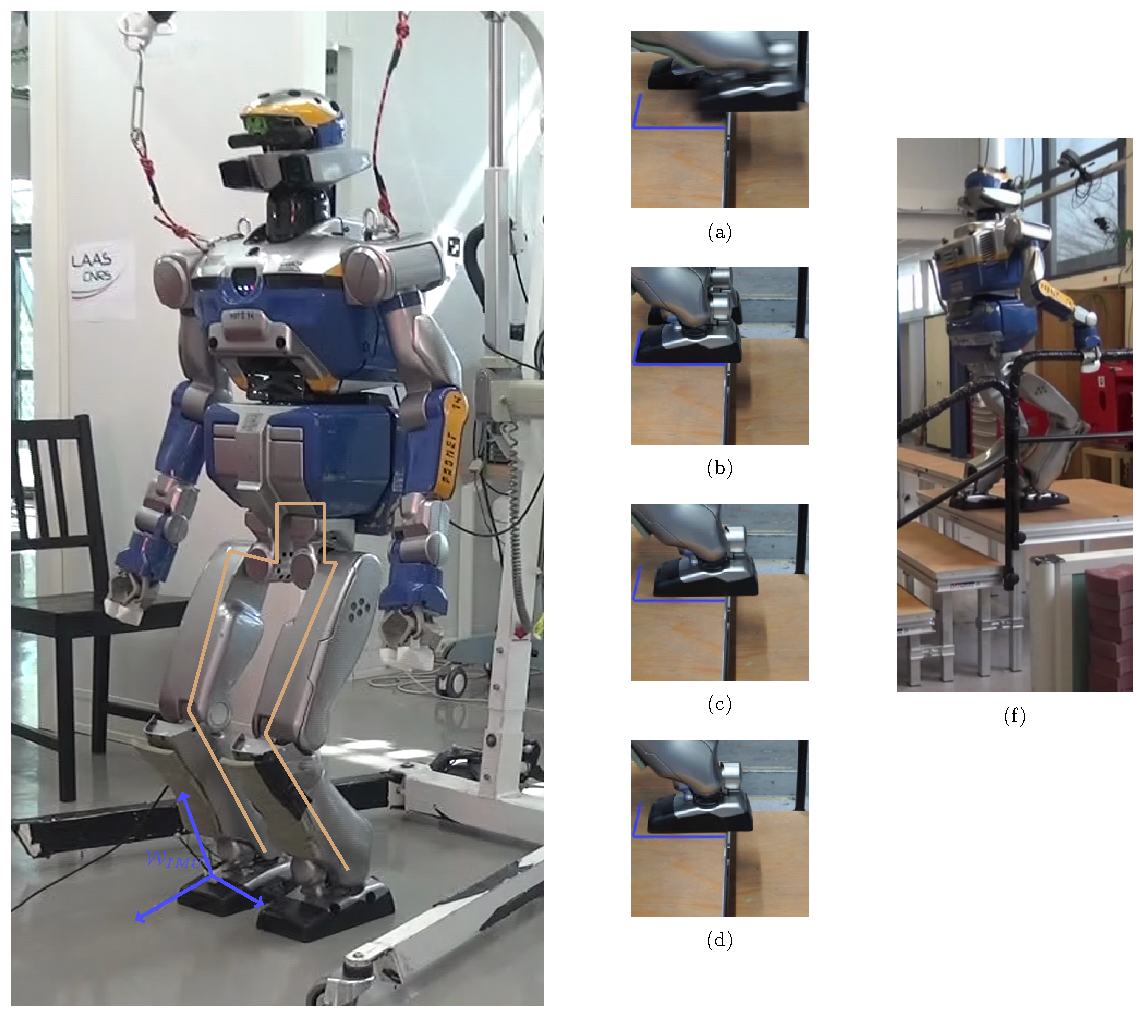
\includegraphics[width=\linewidth]{./figures/cover-figure.pdf}
% 	\caption{D(from \cite{Carpentier:ICRA:2016}).
%  }
% 	\label{fig:cover}
% \end{figure}

\textit{Methodology: }
Graphical methods have been extensively used to implement such fusion strategies \cite{Thrun:ijrr:2006,Kaess:itro:2008}.
They are well-suited to gather information from sensors
and draw conclusions. The underlying principle is to consider that despite all the information gathered from the sensors, we still have uncertainties about the true state of the world due to imperfections of the sensors.
Several states of the world can thus be considered as probable.
Relying on probabilistic formulations is a way find out the most probable one. Furthermore, graphical representation are able to accurately model 
complex estimation problems~\cite{koller2009probabilistic} in a versatile way. 

Graphical models have been used for large modeling estimation problems by means of sparse networks of constraints and particularly in
robotics where SLAM and visual odometry problems have reached a high degree of maturity in great part thanks to these tools.
The graphical representation also allows for the design of powerful nonlinear estimation solvers, which can be built taking into account the needs for accuracy, 
robustness and CPU-performance.

In order to keep the problem tractable and maintain real-time performance a key point is to prevent the graph from being too large given a time window.
IMUs are challenging in this regard, as their high frequency measurement rate create large sets of data. 
Pre-integration of IMU measurements helps to reduce the size of the graph by summarizing 100 to 1000 measures into a single pre-integrated Bayesian node~\cite{LUPTON-09}.
Direct pre-integration leads to a dependency of the resulting node on the initial integration condition, implying to integrate again (and again) when an optimizer process the graph.
It was later suggested to make this pre-integrated data independent from the initial state where it was computed~\cite{forster2015imu}.
Consequently, the IMU measurements can simply be disregarded even when the initial ``pre-integration'' condition changes while the numerical solver optimized the maximum-likelihood trajectory.

\textit{Contributions: }
In this paper, we follow a similar methodology. We define a graphical model where pre-integrated data are added at key-frame instants (about 2Hz), summarizing IMU measurements captured at about 1kHz.
The state that we want to estimate considers the position, orientation and linear velocity (dimension 9) of the IMU attached to the foot, along with the accelerometer and gyroscope biases (both varying in time -- dimension 6).
We also implement the prior knowledge that the foot lands horizontally, by adding Bayesian nodes when the foot lands and takes off.
This prior knowledge make the considered state observable. 
We then use a numerical solver to maximize the likelihood of the measurements and prior knowledge along the past trajectory in a sliding window. 

A first contribution of this paper is to reformulate the method proposed in \cite{forster2015imu} from rotation matrix to quaternion representation
and give a detailed and simpler algebraic derivation.
The second contribution is to apply this method for estimating the human foot-pose during walking.
%% We describe the implementation of this pre-integration scheme in a software implementation of the graphical method.
%% %This implementation would allow to simply add different sensor or additional priors for fusion strategies.
%% We compare the level of accuracy obtained with this method against other methods classicaly used in pedestrian localization.

%% We first describe the implementation of this pre-integration scheme in a software implementation of the graphical method designed to
%% allow users to easily gather information from different sensor for fusion strategies.
The gathered information are then used to get a graphical model-based formulation of the problem. 
Once the formulation is completed, a non-linear least squares optimizer is used to solve the problem and find the most probable solution in the least-square sense \cite{ceres-solver}.





